\documentclass[11pt,a4paper]{article}

%% ── Packages ──────────────────────────────────────────────────────────────
\usepackage[a4paper, top=2.5cm, bottom=2.5cm, left=2.5cm, right=2.5cm]{geometry}
\usepackage[T1]{fontenc}
\usepackage[utf8]{inputenc}
\usepackage{xcolor}
\usepackage{graphicx}
\graphicspath{{img/}}
\usepackage{booktabs}
\usepackage{longtable}
\usepackage{array}
\usepackage{enumitem}
\usepackage{hyperref}
\usepackage{fancyhdr}
\usepackage{titlesec}
\usepackage{tcolorbox}
\usepackage{listings}
\usepackage{multirow}
\usepackage{tabularx}
\usepackage{colortbl}
\usepackage{mdframed}
\usepackage{parskip}

%% ── Colour palette ────────────────────────────────────────────────────────
\definecolor{critred}   {HTML}{C0392B}
\definecolor{highorg}   {HTML}{E67E22}
\definecolor{medyel}    {HTML}{F39C12}
\definecolor{lowblue}   {HTML}{2980B9}
\definecolor{infogreen} {HTML}{27AE60}
\definecolor{darkgray}  {HTML}{2C3E50}
\definecolor{lightgray} {HTML}{ECF0F1}
\definecolor{accent}    {HTML}{1A252F}
\definecolor{codebg}    {HTML}{F8F8F8}
\definecolor{codefg}    {HTML}{2C3E50}

%% ── Hyperref ──────────────────────────────────────────────────────────────
\hypersetup{
  colorlinks=true,
  linkcolor=darkgray,
  urlcolor=lowblue,
  citecolor=darkgray,
  pdfauthor={Eyad},
  pdftitle={VAmPI API Penetration Test Report},
}

%% ── Header / Footer ──────────────────────────────────────────────────────
\pagestyle{fancy}
\fancyhf{}
\renewcommand{\headrulewidth}{0.4pt}
\renewcommand{\footrulewidth}{0.4pt}
\fancyhead[L]{\small\textcolor{darkgray}{\textbf{VAmPI API -- Penetration Test Report}}}
\fancyhead[R]{\small\textcolor{darkgray}{CONFIDENTIAL}}
\fancyfoot[L]{\small\textcolor{darkgray}{Eyad -- DEPI Vulnerability Analyst Track}}
\fancyfoot[R]{\small\thepage}

%% ── Section styling ───────────────────────────────────────────────────────
\titleformat{\section}
  {\large\bfseries\color{darkgray}}
  {\thesection}{1em}{}[\titlerule]

\titleformat{\subsection}
  {\normalsize\bfseries\color{darkgray}}
  {\thesubsection}{1em}{}

%% ── Listings (code) ──────────────────────────────────────────────────────
\lstset{
  backgroundcolor=\color{codebg},
  basicstyle=\ttfamily\footnotesize\color{codefg},
  breaklines=true,
  frame=single,
  framesep=4pt,
  rulecolor=\color{lightgray},
  xleftmargin=8pt,
  xrightmargin=8pt,
}

%% ── Severity badge helper ─────────────────────────────────────────────────
\newcommand{\critical}[1]{\colorbox{critred}{\color{white}\textbf{\footnotesize #1}}}
\newcommand{\high}[1]   {\colorbox{highorg}{\color{white}\textbf{\footnotesize #1}}}
\newcommand{\medium}[1] {\colorbox{medyel} {\color{white}\textbf{\footnotesize #1}}}
\newcommand{\low}[1]    {\colorbox{lowblue}{\color{white}\textbf{\footnotesize #1}}}
\newcommand{\info}[1]   {\colorbox{infogreen}{\color{white}\textbf{\footnotesize #1}}}

%% ── Finding box ──────────────────────────────────────────────────────────
\newenvironment{findingbox}[2]{%
  \begin{tcolorbox}[
    colback=lightgray,
    colframe=darkgray,
    title={\textbf{#1} \hfill #2},
    fonttitle=\small,
    arc=2pt,
    boxrule=0.5pt,
    left=6pt, right=6pt, top=4pt, bottom=4pt
  ]
}{%
  \end{tcolorbox}
}

%% ── Document ──────────────────────────────────────────────────────────────
\begin{document}

%% ── Cover Page ────────────────────────────────────────────────────────────
\begin{titlepage}
  \pagecolor{accent}
  \color{white}
  \centering
  \vspace*{3cm}

  {\Huge\bfseries VAmPI REST API}\\[0.4cm]
  {\LARGE Penetration Test Report}\\[1.2cm]
  \rule{10cm}{0.4pt}\\[1.2cm]

  \begin{tabular}{rl}
    \textbf{Target}     & VAmPI -- Vulnerable API \\
    \textbf{Version}    & Docker (erev0s/VAmPI) \\
    \textbf{Date}       & November 2026 \\
    \textbf{By}         & Eyad Islam El-Taher \\
    \textbf{Track}      & Vulnerability Analyst \& Penetration Tester \\
  \end{tabular}

  \vfill
  \rule{10cm}{0.4pt}\\[0.3cm]
  {\small This document is intended solely for authorised recipients.}
\end{titlepage}
\pagecolor{white}\color{black}

\tableofcontents
\newpage

%% ═══════════════════════════════════════════════════════════════════════════
\section{Executive Summary}
%% ═══════════════════════════════════════════════════════════════════════════

A penetration test was conducted against \textbf{VAmPI}, an intentionally vulnerable REST API running locally via Docker. The assessment covered all documented endpoints and focused on the OWASP API Security Top 10 vulnerability classes.

\textbf{Eleven (11) vulnerabilities} were identified across five severity levels. Critical and High findings allow full account takeover, privilege escalation to administrator, and complete database exfiltration without authentication.

\vspace{0.5em}
\begin{center}
\begin{tabular}{lcc}
  \toprule
  \textbf{Severity} & \textbf{Count} & \textbf{CVSS Range} \\
  \midrule
  \rowcolor{critred!15} Critical & 2 & 9.0 -- 10.0 \\
  \rowcolor{highorg!15} High     & 4 & 7.0 -- 8.9  \\
  \rowcolor{medyel!15}  Medium   & 3 & 4.0 -- 6.9  \\
  \rowcolor{lowblue!15} Low      & 2 & 0.1 -- 3.9  \\
  \midrule
  \textbf{Total}   & \textbf{11} & \\
  \bottomrule
\end{tabular}
\end{center}

%% ═══════════════════════════════════════════════════════════════════════════
\section{Scope \& Methodology}
%% ═══════════════════════════════════════════════════════════════════════════

\subsection{Scope}

\begin{center}
\begin{tabularx}{\textwidth}{llX}
  \toprule
  \textbf{Method} & \textbf{Endpoint} & \textbf{Description} \\
  \midrule
  GET  & \texttt{/createdb}                       & Creates and populates the database \\
  GET  & \texttt{/}                               & VAmPI home \\
  GET  & \texttt{/me}                             & Current authenticated user \\
  GET  & \texttt{/users/v1}                       & List all users (basic info) \\
  GET  & \texttt{/users/v1/\_debug}               & List all users (full details) \\
  POST & \texttt{/users/v1/register}              & Register new user \\
  POST & \texttt{/users/v1/login}                 & Authenticate user \\
  GET  & \texttt{/users/v1/\{username\}}          & Get user by username \\
  DELETE & \texttt{/users/v1/\{username\}}        & Delete user (admin only) \\
  PUT  & \texttt{/users/v1/\{username\}/email}    & Update user email \\
  PUT  & \texttt{/users/v1/\{username\}/password} & Update user password \\
  GET  & \texttt{/books/v1}                       & List all books \\
  POST & \texttt{/books/v1}                       & Add new book \\
  GET  & \texttt{/books/v1/\{book\}}              & Get book with secret content \\
  \bottomrule
\end{tabularx}
\end{center}

\subsection{Methodology}

Testing followed a black-box approach using manual analysis and automated tooling. Tools used: \textbf{Burp Suite} (interception, Intruder), \textbf{Postman} (API interaction), \textbf{sqlmap} (SQL injection), \textbf{hashcat} (JWT cracking), \textbf{jwt.io} (token analysis).

Vulnerabilities are categorised per the \textbf{OWASP API Security Top 10 (2023)}.

%% ═══════════════════════════════════════════════════════════════════════════
\section{Findings Summary}
%% ═══════════════════════════════════════════════════════════════════════════

\begin{center}
\begin{tabularx}{\textwidth}{clXll}
  \toprule
  \textbf{\#} & \textbf{Title} & \textbf{Endpoint} & \textbf{OWASP} & \textbf{Severity} \\
  \midrule
  1 & SQL Injection           & \texttt{/users/v1/*}         & API8:2023 & \critical{CRITICAL} \\
  2 & JWT Weak Secret         & \texttt{/users/v1/login}     & API2:2023 & \critical{CRITICAL} \\
  3 & Mass Assignment         & \texttt{/users/v1/register}  & API6:2023 & \high{HIGH} \\
  4 & Unauthorized Password Change & \texttt{/users/v1/\{u\}/pass} & API1:2023 & \high{HIGH} \\
  5 & BOLA on Books           & \texttt{/books/v1/\{book\}}  & API1:2023 & \high{HIGH} \\
  6 & Brute Force / No Rate Limiting & \texttt{/users/v1/login} & API4:2023 & \high{HIGH} \\
  7 & Debug Endpoint Exposure & \texttt{/users/v1/\_debug}   & API9:2023 & \medium{MEDIUM} \\
  8 & Information Disclosure (SQLi Error) & \texttt{/users/v1/\{u\}} & API9:2023 & \medium{MEDIUM} \\
  9 & User \& Password Enumeration & \texttt{/users/v1}      & API9:2023 & \medium{MEDIUM} \\
  10 & Missing Email Validation & \texttt{/users/v1/register} & API3:2023 & \low{LOW} \\
  11 & Weak Password Policy    & \texttt{/users/v1/register}  & API3:2023 & \low{LOW} \\
  \bottomrule
\end{tabularx}
\end{center}

\newpage
%% ═══════════════════════════════════════════════════════════════════════════
\section{Detailed Findings}
%% ═══════════════════════════════════════════════════════════════════════════

%% ─── Finding 1 ───────────────────────────────────────────────────────────
\subsection{VULN-01 -- SQL Injection}

\begin{findingbox}{VULN-01: SQL Injection}{\critical{CRITICAL}}
\begin{tabular}{ll}
  \textbf{Endpoint}   & \texttt{GET /users/v1/\{username\}} \\
  \textbf{OWASP}      & API8:2023 -- Security Misconfiguration \\
  \textbf{CVSS Score} & 9.8 (AV:N/AC:L/PR:N/UI:N/S:U/C:H/I:H/A:H) \\
\end{tabular}
\end{findingbox}

\textbf{Description.}
The \texttt{username} path parameter is passed directly into an SQL query without sanitisation. Appending a single quote to the username causes the SQLite backend to throw a raw exception, confirming unsanitised input. Using \texttt{sqlmap} with a wildcard payload against \texttt{/users/v1/*} allowed full database dump without authentication.

\textbf{Proof of Concept.}
\begin{lstlisting}
# Single-quote injection triggers 500 + raw SQL error
GET /users/v1/eyad'
# -> 500: sqlalchemy.exc.OperationalError: unrecognized token: "'eyad''"
#    SQL: SELECT * FROM users WHERE username = 'eyad''

# sqlmap full dump
sqlmap -u "http://127.0.0.1:5000/users/v1/*" \
       --dbms=sqlite --dump-all --risk=2 --level=2
\end{lstlisting}

\begin{figure}[h!]
  \centering
  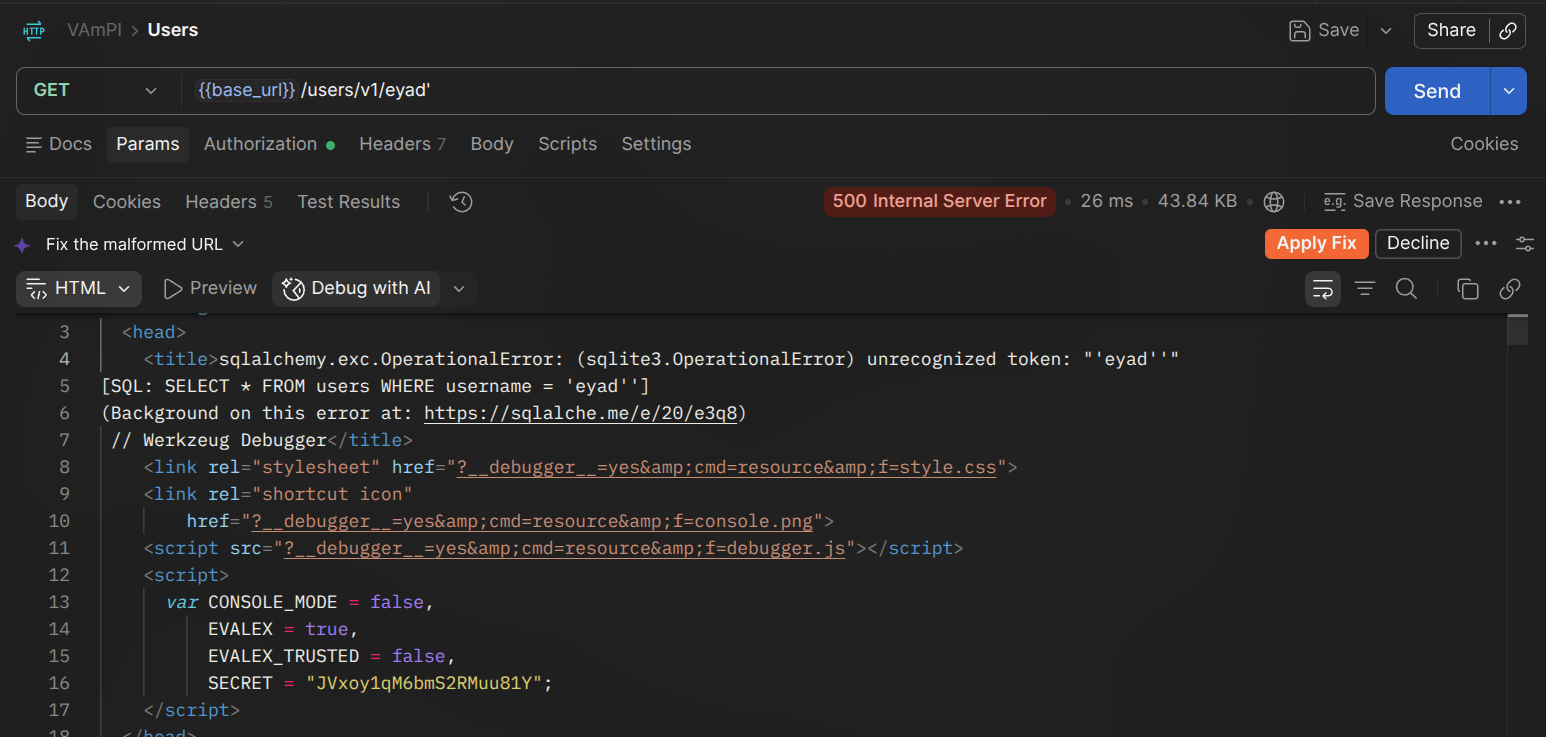
\includegraphics[width=0.92\textwidth]{information disclosure.png}
  \caption{Raw SQL error returned to client on malformed username}
\end{figure}

\begin{figure}[h!]
  \centering
  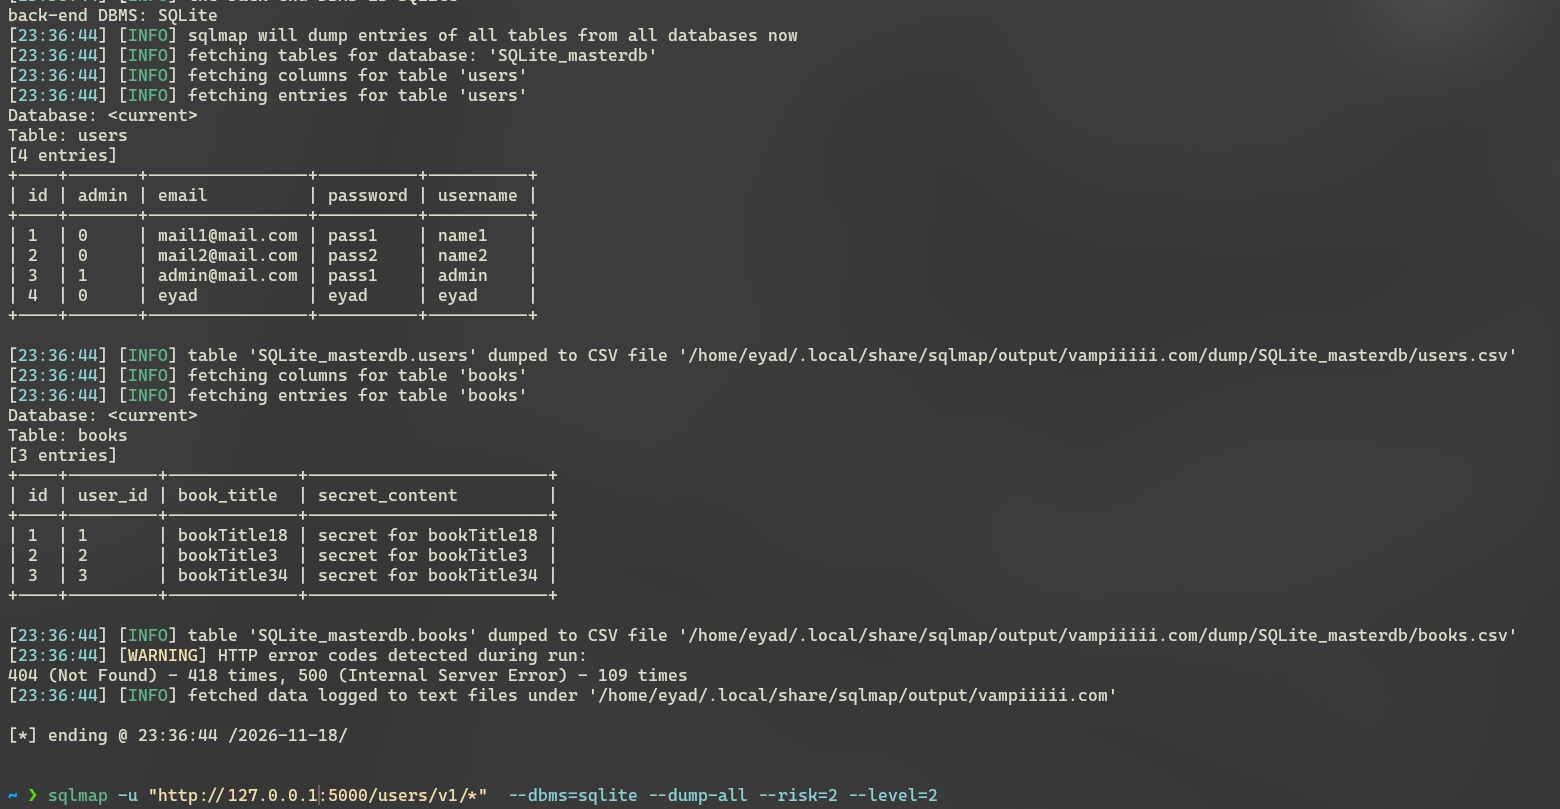
\includegraphics[width=0.92\textwidth]{SQLi.png}
  \caption{sqlmap dumps full \texttt{users} and \texttt{books} tables including plaintext passwords and secret book content}
\end{figure}

\textbf{Impact.} Complete exfiltration of all user credentials and book secrets. Credentials are stored in plaintext, so no further cracking is required.

\textbf{Remediation.}
\begin{itemize}[noitemsep]
  \item Use parameterised queries / ORM bound parameters exclusively.
  \item Disable debug mode in production; never return raw exception traces to the client.
  \item Implement a WAF rule blocking common SQLi patterns.
\end{itemize}

\vspace*{10cm}
\newpage
\newpage

%% ─── Finding 2 ───────────────────────────────────────────────────────────
\subsection{VULN-02 -- JWT Weak Secret}

\begin{findingbox}{VULN-02: JWT Signed with Weak Secret}{\critical{CRITICAL}}
\begin{tabular}{ll}
  \textbf{Endpoint}   & \texttt{POST /users/v1/login} (token issuance) \\
  \textbf{OWASP}      & API2:2023 -- Broken Authentication \\
  \textbf{CVSS Score} & 9.1 (AV:N/AC:L/PR:N/UI:N/S:U/C:H/I:H/A:N) \\
\end{tabular}
\end{findingbox}

\textbf{Description.}
Access tokens are JWT HS256. The signing secret was recovered in under one second using \texttt{hashcat} mode 16500 against \texttt{rockyou.txt}. Possession of the secret allows an attacker to forge arbitrary tokens -- including admin-privileged ones -- for any user.

\textbf{Proof of Concept.}
\begin{lstlisting}
hashcat -m 16500 <jwt> /usr/share/wordlists/rockyou.txt
# Status: Cracked  (0 seconds)
# Secret recovered: "secret1"   (found in rockyou.txt)
\end{lstlisting}

\begin{figure}[h!]
  \centering
  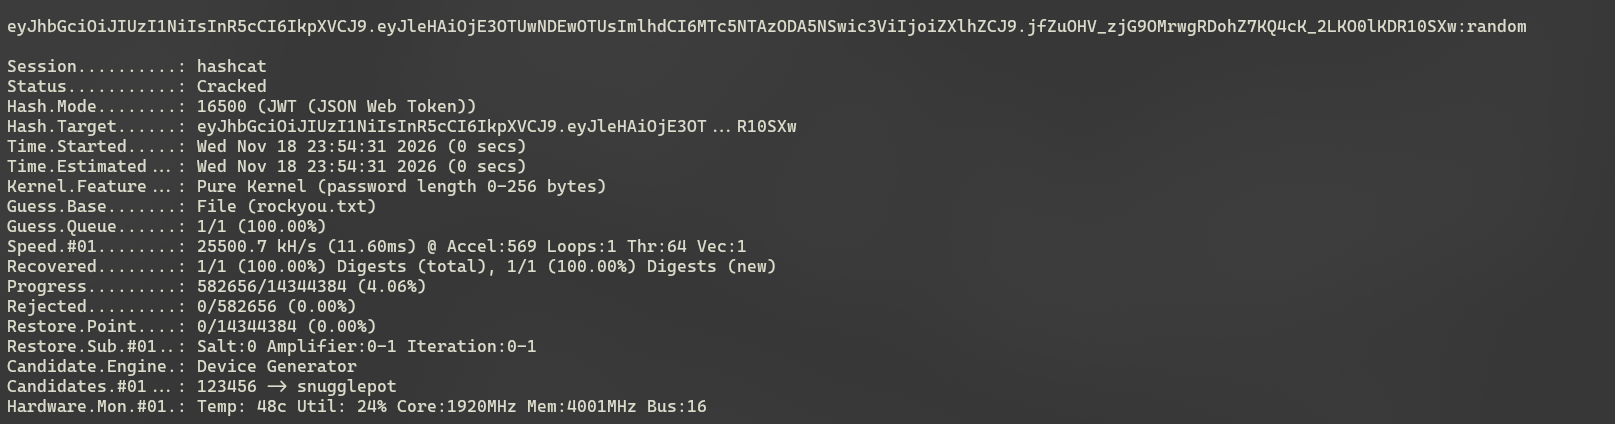
\includegraphics[width=0.92\textwidth]{jwt weak secret.png}
  \caption{hashcat cracks the JWT HS256 secret from rockyou.txt in under one second}
\end{figure}

\textbf{Impact.} Full authentication bypass; arbitrary privilege escalation; persistent session hijacking for all users.

\textbf{Remediation.}
\begin{itemize}[noitemsep]
  \item Generate the JWT secret from a CSPRNG with at least 256 bits of entropy.
  \item Rotate the secret immediately if compromise is suspected.
  \item Consider RS256/ES256 (asymmetric) so the signing key never leaves the server.
\end{itemize}

\newpage
%% ─── Finding 3 ───────────────────────────────────────────────────────────
\subsection{VULN-03 -- Mass Assignment (Privilege Escalation to Admin)}

\begin{findingbox}{VULN-03: Mass Assignment}{\high{HIGH}}
\begin{tabular}{ll}
  \textbf{Endpoint}   & \texttt{POST /users/v1/register} \\
  \textbf{OWASP}      & API6:2023 -- Unrestricted Access to Sensitive Business Flows \\
  \textbf{CVSS Score} & 8.8 (AV:N/AC:L/PR:L/UI:N/S:U/C:H/I:H/A:N) \\
\end{tabular}
\end{findingbox}

\textbf{Description.}
The registration endpoint binds the entire request body to the user model without filtering internal fields. Supplying \texttt{"admin": true} in the JSON body creates an account with administrator privileges.

\textbf{Proof of Concept.}
\begin{lstlisting}
POST /users/v1/register
{"username":"eyadAsAdmin","password":"eyad","email":"eyad","admin": true}
# -> 200 OK: "Successfully registered."

GET /me  (with eyadAsAdmin token)
# -> {"admin": true, "email": "eyad", "username": "eyadAsAdmin"}
\end{lstlisting}

\begin{figure}[h!]
  \centering
  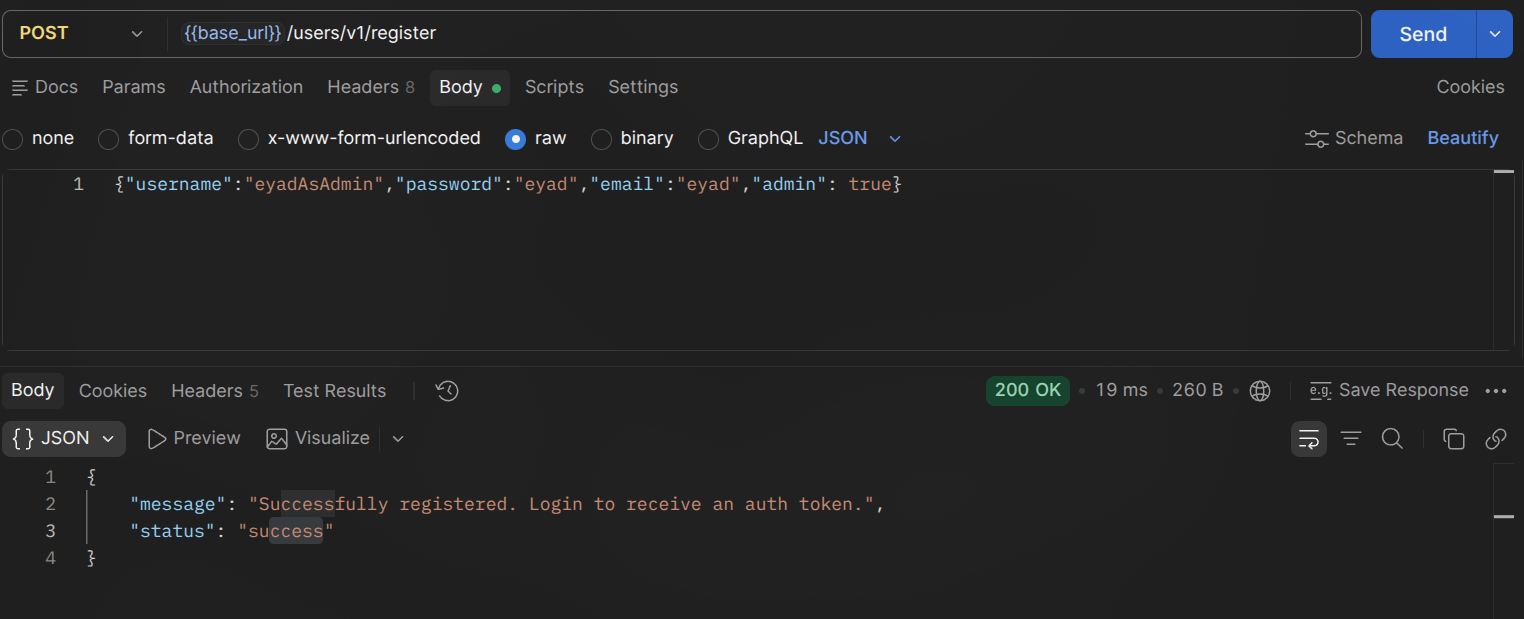
\includegraphics[width=0.88\textwidth]{massAssignment.png}
  \caption{Registration request injecting \texttt{"admin": true}}
\end{figure}

\begin{figure}[h!]
  \centering
  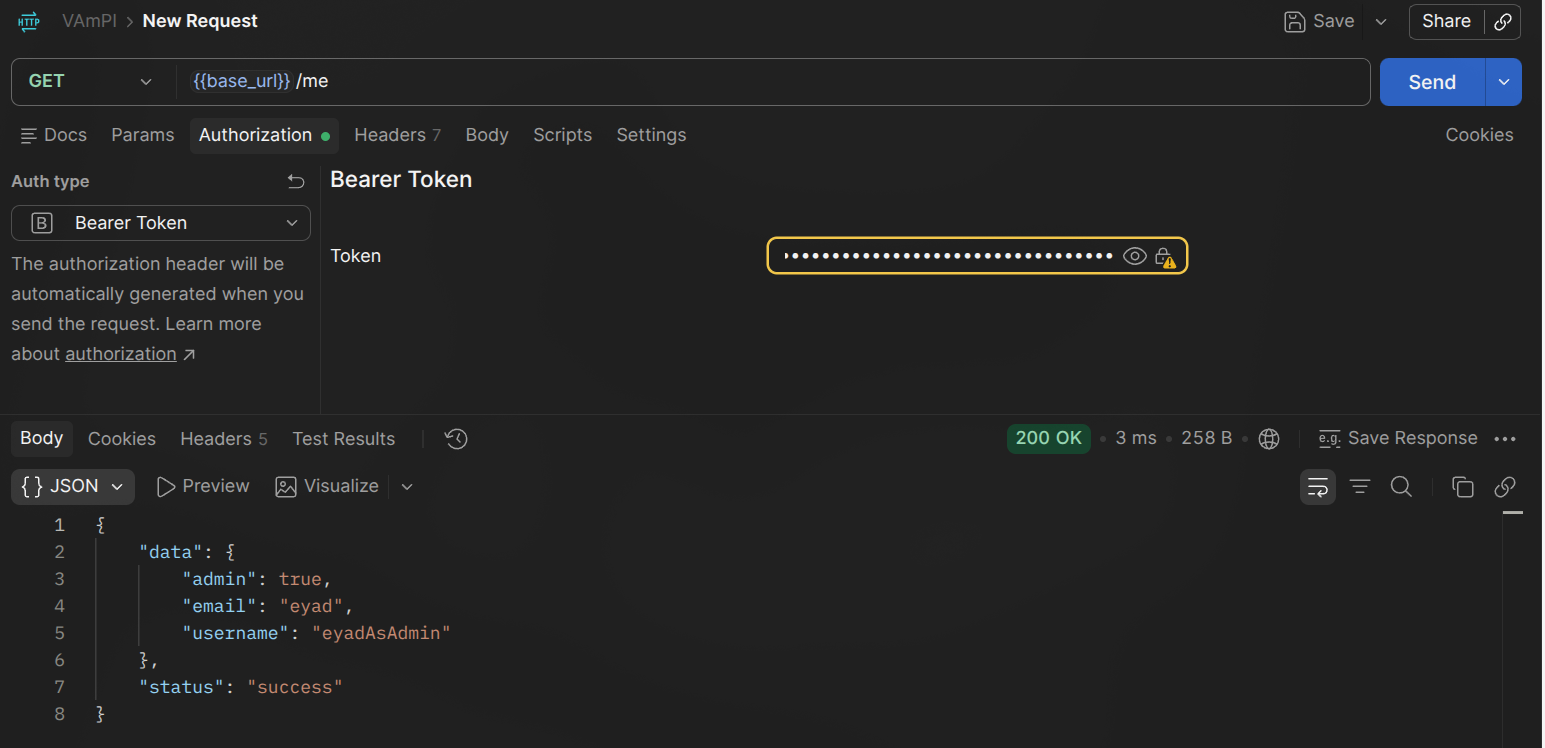
\includegraphics[width=0.88\textwidth]{massAssignment2(logged in as admin).png}
  \caption{\texttt{/me} confirms the new account holds admin privileges}
\end{figure}

\textbf{Impact.} Any unauthenticated user can self-grant administrator access, defeating all role-based access controls.

\textbf{Remediation.}
\begin{itemize}[noitemsep]
  \item Use an explicit allowlist of accepted registration fields; strip or reject any unlisted fields.
  \item Never bind HTTP input directly to internal model objects (avoid mass assignment patterns).
\end{itemize}

\newpage
%% ─── Finding 4 ───────────────────────────────────────────────────────────
\subsection{VULN-04 -- Unauthorized Password Change (BOLA/BFLA)}

\begin{findingbox}{VULN-04: Unauthorized Password Change}{\high{HIGH}}
\begin{tabular}{ll}
  \textbf{Endpoint}   & \texttt{PUT /users/v1/\{username\}/password} \\
  \textbf{OWASP}      & API1:2023 -- Broken Object Level Authorization \\
  \textbf{CVSS Score} & 8.1 (AV:N/AC:L/PR:L/UI:N/S:U/C:N/I:H/A:H) \\
\end{tabular}
\end{findingbox}

\textbf{Description.}
The password update endpoint does not verify that the authenticated user owns the target account. Any authenticated user can change another user's password by substituting a different username in the URL path.

\textbf{Proof of Concept.}
\begin{enumerate}[noitemsep]
  \item Authenticate as \texttt{eyad}; obtain JWT.
  \item Send \texttt{PUT /users/v1/name1/password} with \texttt{eyad}'s token and body \texttt{\{"password":"pass"\}}.
  \item Server returns \texttt{204 No Content} -- password changed.
  \item Login as \texttt{name1} with the new password succeeds.
\end{enumerate}

\begin{figure}[h!]
  \centering
  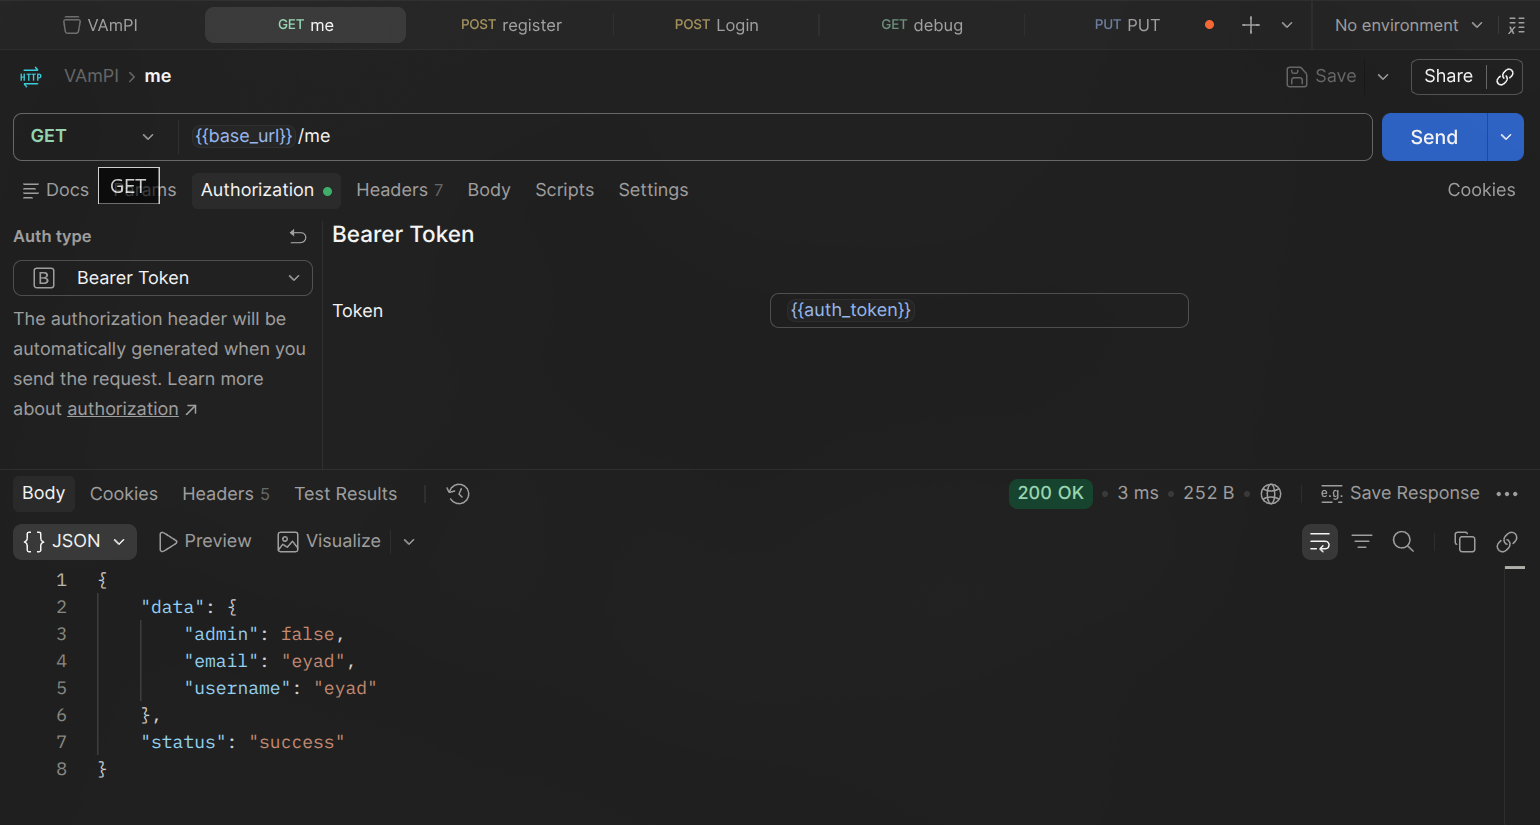
\includegraphics[width=0.88\textwidth]{Unauthorized Password Change_1.png}
  \caption{Step 1 -- \texttt{/me} confirms authenticated as \texttt{eyad} (admin: false)}
\end{figure}

\begin{figure}[h!]
  \centering
  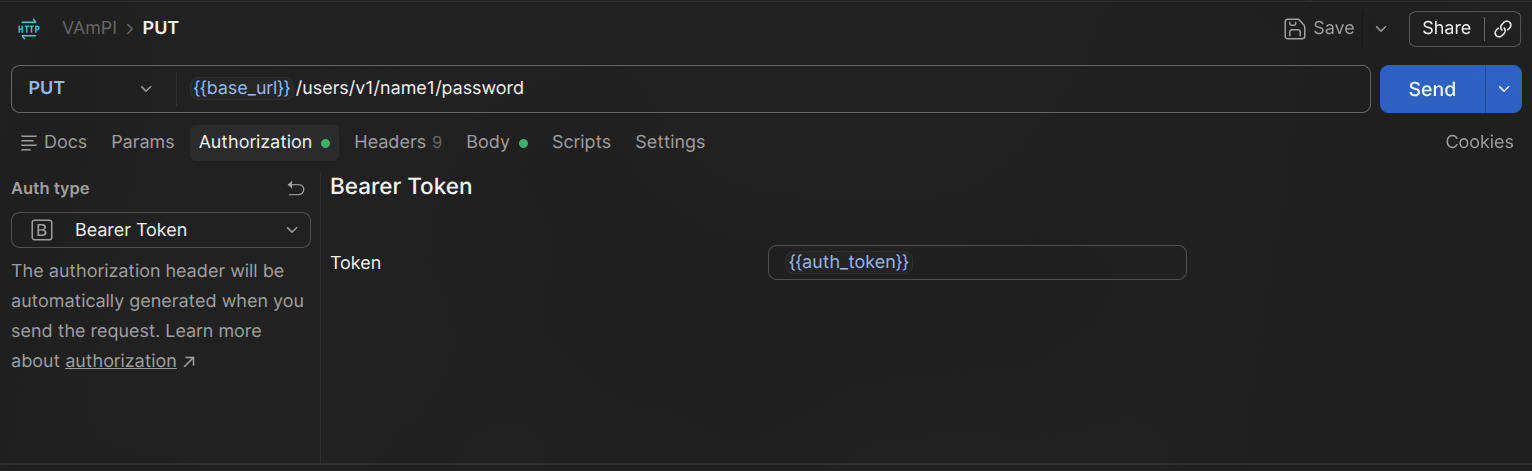
\includegraphics[width=0.88\textwidth]{Unauthorized Password Change_2.png}
  \caption{Step 2 -- PUT to \texttt{name1/password} using \texttt{eyad}'s token}
\end{figure}

\begin{figure}[h!]
  \centering
  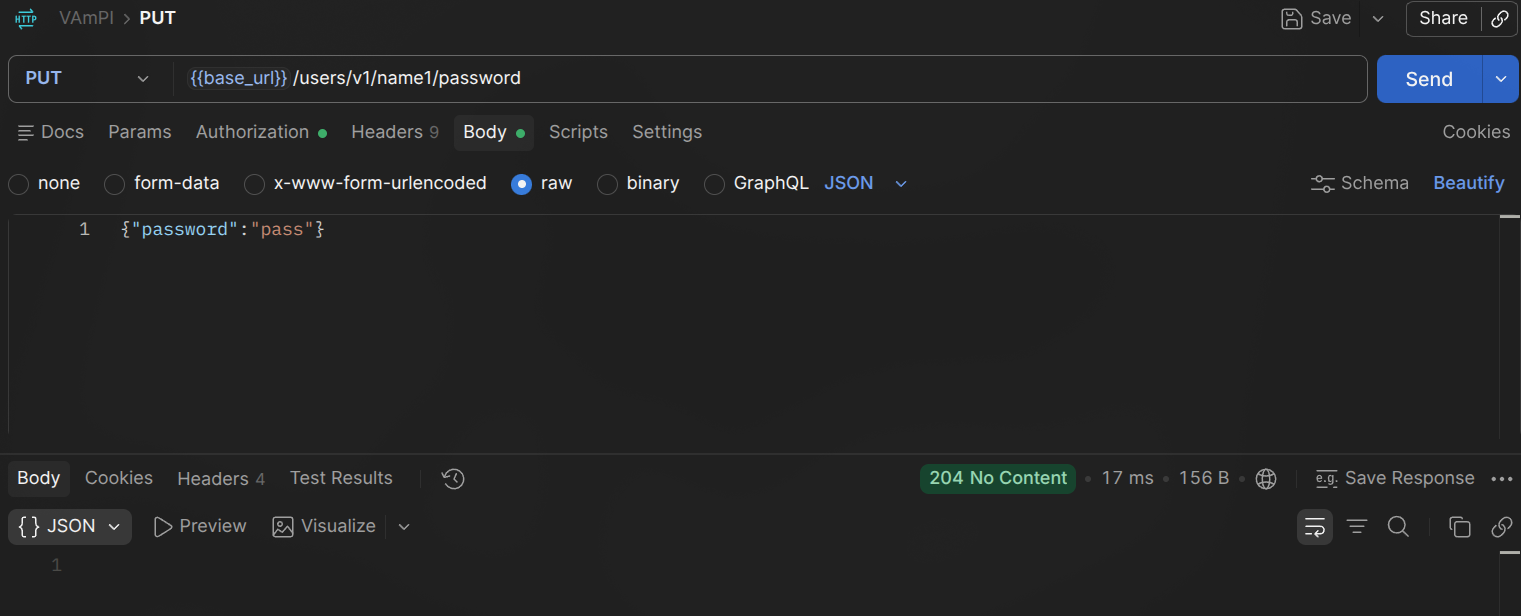
\includegraphics[width=0.88\textwidth]{Unauthorized Password Change_3.png}
  \caption{Step 3 -- Server responds 204, password changed}
\end{figure}

\begin{figure}[h!]
  \centering
  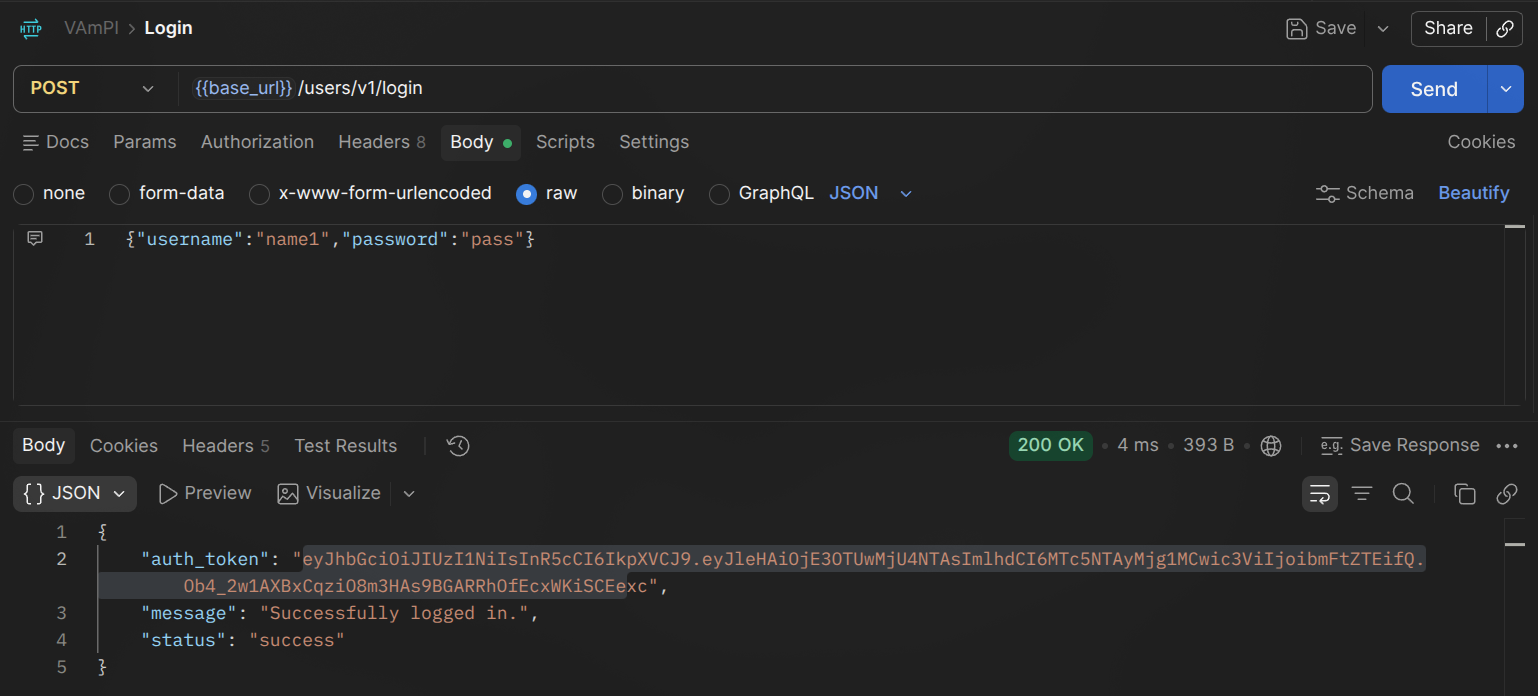
\includegraphics[width=0.88\textwidth]{Unauthorized Password Change_4.png}
  \caption{Step 4 -- \texttt{name1} logs in with the attacker-set password}
\end{figure}

\textbf{Impact.} Full account takeover for any user. Combined with admin enumeration from \texttt{/users/v1}, an attacker can take over administrator accounts.

\textbf{Remediation.}
\begin{itemize}[noitemsep]
  \item Enforce object-level authorisation: compare the token's \texttt{sub}/username claim against the path parameter before processing.
  \item Require current-password confirmation for password change operations.
\end{itemize}

\newpage
%% ─── Finding 5 ───────────────────────────────────────────────────────────
\subsection{VULN-05 -- Broken Object Level Authorization (BOLA) on Books}

\begin{findingbox}{VULN-05: BOLA -- Unauthorized Book Secret Access}{\high{HIGH}}
\begin{tabular}{ll}
  \textbf{Endpoint}   & \texttt{GET /books/v1/\{book\_title\}} \\
  \textbf{OWASP}      & API1:2023 -- Broken Object Level Authorization \\
  \textbf{CVSS Score} & 7.5 (AV:N/AC:L/PR:L/UI:N/S:U/C:H/I:N/A:N) \\
\end{tabular}
\end{findingbox}

\textbf{Description.}
The book detail endpoint returns the \texttt{secret\_content} field for any book title regardless of whether the requesting user owns that book. Any authenticated user can retrieve another user's private book secrets by guessing or enumerating book titles.

\textbf{Proof of Concept.}
\begin{lstlisting}
# Authenticated as eyad (owns no books)
GET /books/v1/bookTitle18
Authorization: Bearer <eyad_token>
# -> 200 OK
# {"book_title":"bookTitle18","owner":"name1","secret":"secret for bookTitle18"}
\end{lstlisting}

\begin{figure}[h!]
  \centering
  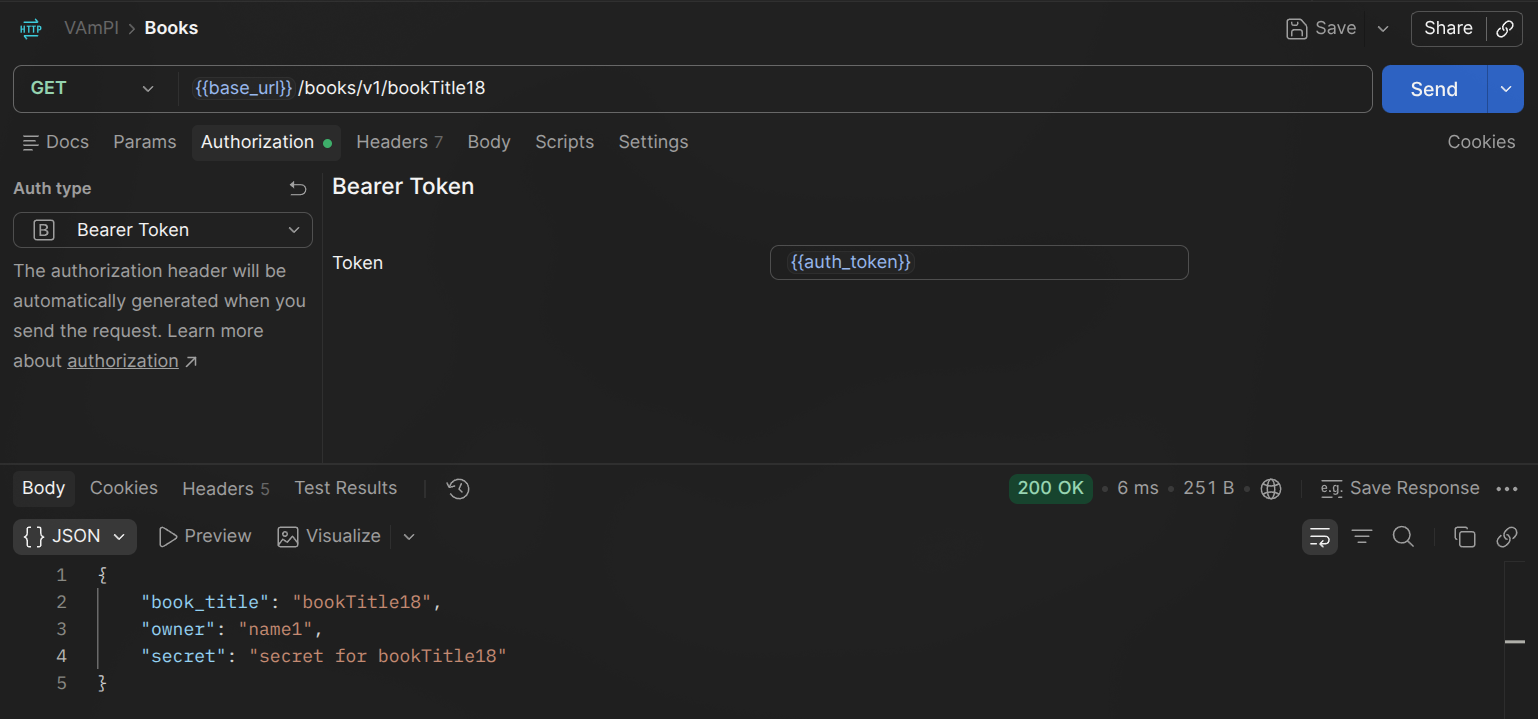
\includegraphics[width=0.92\textwidth]{BOLA.png}
  \caption{\texttt{eyad} retrieves the secret of \texttt{bookTitle18} owned by \texttt{name1}}
\end{figure}

\textbf{Impact.} Confidential content of every book in the system is accessible to any authenticated user.

\textbf{Remediation.}
\begin{itemize}[noitemsep]
  \item Verify \texttt{book.owner == request.user} before returning \texttt{secret\_content}.
  \item Omit sensitive fields from the response object for non-owner requests.
\end{itemize}

\newpage
%% ─── Finding 6 ───────────────────────────────────────────────────────────
\subsection{VULN-06 -- No Rate Limiting / Brute Force on Login}

\begin{findingbox}{VULN-06: Lack of Rate Limiting -- Brute Force}{\high{HIGH}}
\begin{tabular}{ll}
  \textbf{Endpoint}   & \texttt{POST /users/v1/login} \\
  \textbf{OWASP}      & API4:2023 -- Unrestricted Resource Consumption \\
  \textbf{CVSS Score} & 7.5 (AV:N/AC:L/PR:N/UI:N/S:U/C:H/I:N/A:N) \\
\end{tabular}
\end{findingbox}

\textbf{Description.}
The login endpoint imposes no rate limit, lockout, or CAPTCHA. Using Burp Suite Intruder with a password wordlist, the \texttt{admin} account password (\texttt{pass1}) was recovered via brute force (request \#3425 in the attack run).

\textbf{Proof of Concept.}
\begin{lstlisting}
# Burp Intruder -- Sniper attack on password field
POST /users/v1/login  {"username":"admin","password":"§FUZZ§"}
# Request 3425: password=pass1  -> 200 OK, auth_token returned
\end{lstlisting}

\begin{figure}[h!]
  \centering
  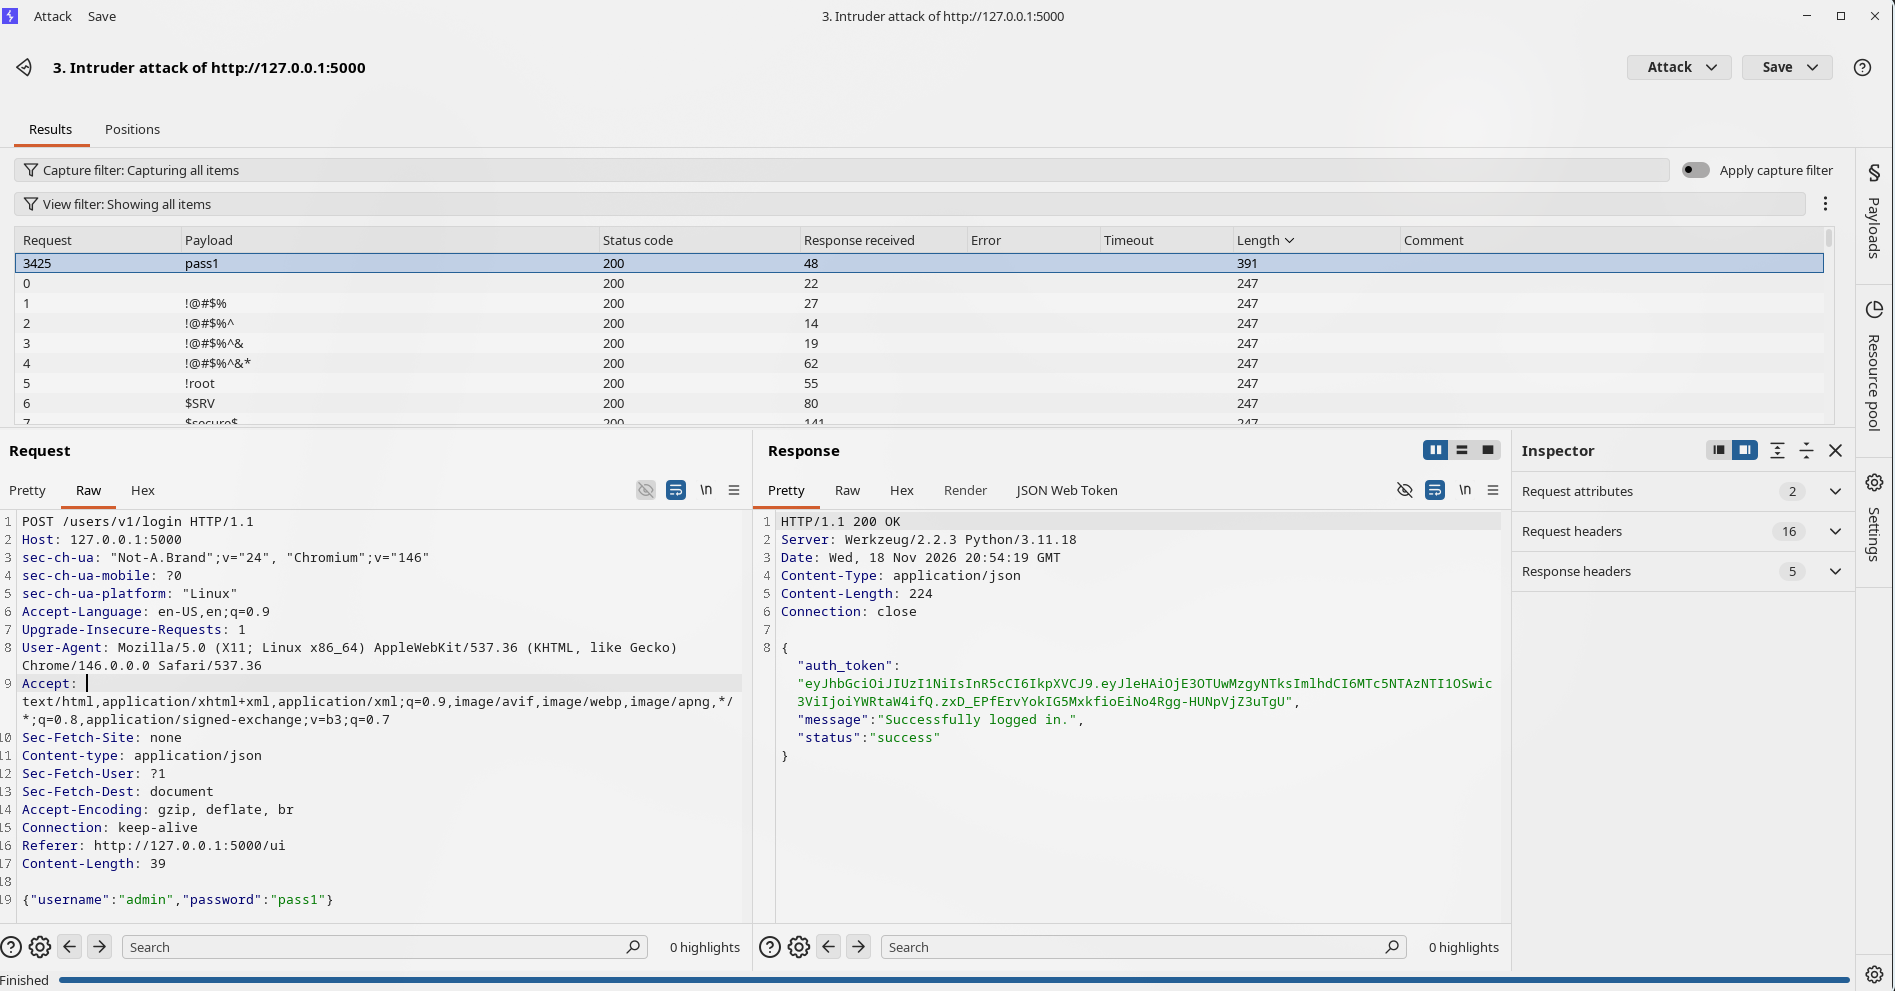
\includegraphics[width=0.92\textwidth]{bruteforceOnWeakPassowrdPolicy.png}
  \caption{Burp Intruder results -- request 3425 with payload \texttt{pass1} returns a longer response (391 B) indicating successful authentication}
\end{figure}

\textbf{Impact.} Offline or online brute force of any account. Combined with weak passwords (Finding 11), this is trivially exploitable.

\textbf{Remediation.}
\begin{itemize}[noitemsep]
  \item Implement exponential back-off and account lockout after $n$ failed attempts.
  \item Apply IP-based and account-based rate limiting (e.g.\ 5 attempts / minute).
  \item Log and alert on repeated authentication failures.
\end{itemize}

\newpage
%% ─── Finding 7 ───────────────────────────────────────────────────────────
\subsection{VULN-07 -- Unauthenticated Debug Endpoint}

\begin{findingbox}{VULN-07: Debug Endpoint Exposes All User Data}{\medium{MEDIUM}}
\begin{tabular}{ll}
  \textbf{Endpoint}   & \texttt{GET /users/v1/\_debug} \\
  \textbf{OWASP}      & API9:2023 -- Improper Inventory Management \\
  \textbf{CVSS Score} & 6.5 (AV:N/AC:L/PR:N/UI:N/S:U/C:H/I:N/A:N) \\
\end{tabular}
\end{findingbox}

\textbf{Description.}
The \texttt{/\_debug} endpoint returns the full user list including plaintext passwords and admin flags, with no authentication required.

\textbf{Proof of Concept.}
\begin{lstlisting}
GET /users/v1/_debug   (no token)
# -> 200 OK
# [{"admin":false,"email":"mail1@mail.com","password":"pass","username":"name1"},
#  {"admin":true, "email":"admin@mail.com","password":"pass1","username":"admin"},
#  ...]
\end{lstlisting}

\begin{figure}[h!]
  \centering
  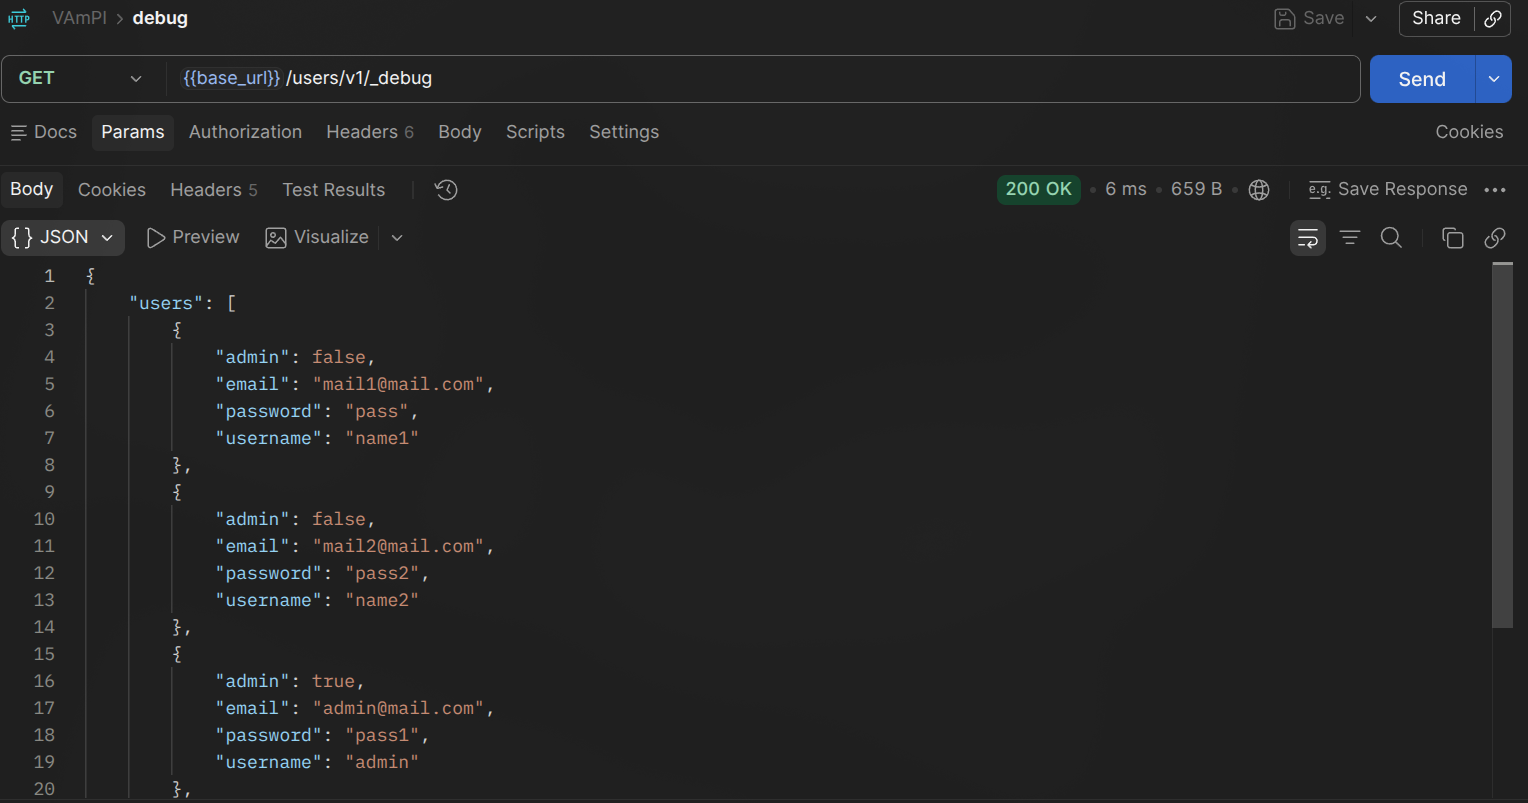
\includegraphics[width=0.92\textwidth]{_debug.png}
  \caption{\texttt{/users/v1/\_debug} returns all credentials without authentication}
\end{figure}

\textbf{Impact.} Immediate access to all usernames, plaintext passwords, emails, and admin status -- instant full compromise.

\textbf{Remediation.}
\begin{itemize}[noitemsep]
  \item Remove debug endpoints entirely from production builds.
  \item Gate any internal diagnostic routes behind admin authentication and restrict by IP.
\end{itemize}

\newpage
%% ─── Finding 8 ───────────────────────────────────────────────────────────
\subsection{VULN-08 -- Information Disclosure via Error Messages}

\begin{findingbox}{VULN-08: Verbose SQL Errors Leaked to Client}{\medium{MEDIUM}}
\begin{tabular}{ll}
  \textbf{Endpoint}   & \texttt{GET /users/v1/\{username\}} \\
  \textbf{OWASP}      & API9:2023 -- Improper Inventory Management \\
  \textbf{CVSS Score} & 5.3 (AV:N/AC:L/PR:N/UI:N/S:U/C:L/I:N/A:N) \\
\end{tabular}
\end{findingbox}

\textbf{Description.}
Injecting a single quote into the username path parameter triggers a 500 response containing the raw SQL query, database type (SQLite), ORM details (SQLAlchemy), and the Werkzeug debug secret. This information directly enables VULN-01.

\begin{figure}[h!]
  \centering
  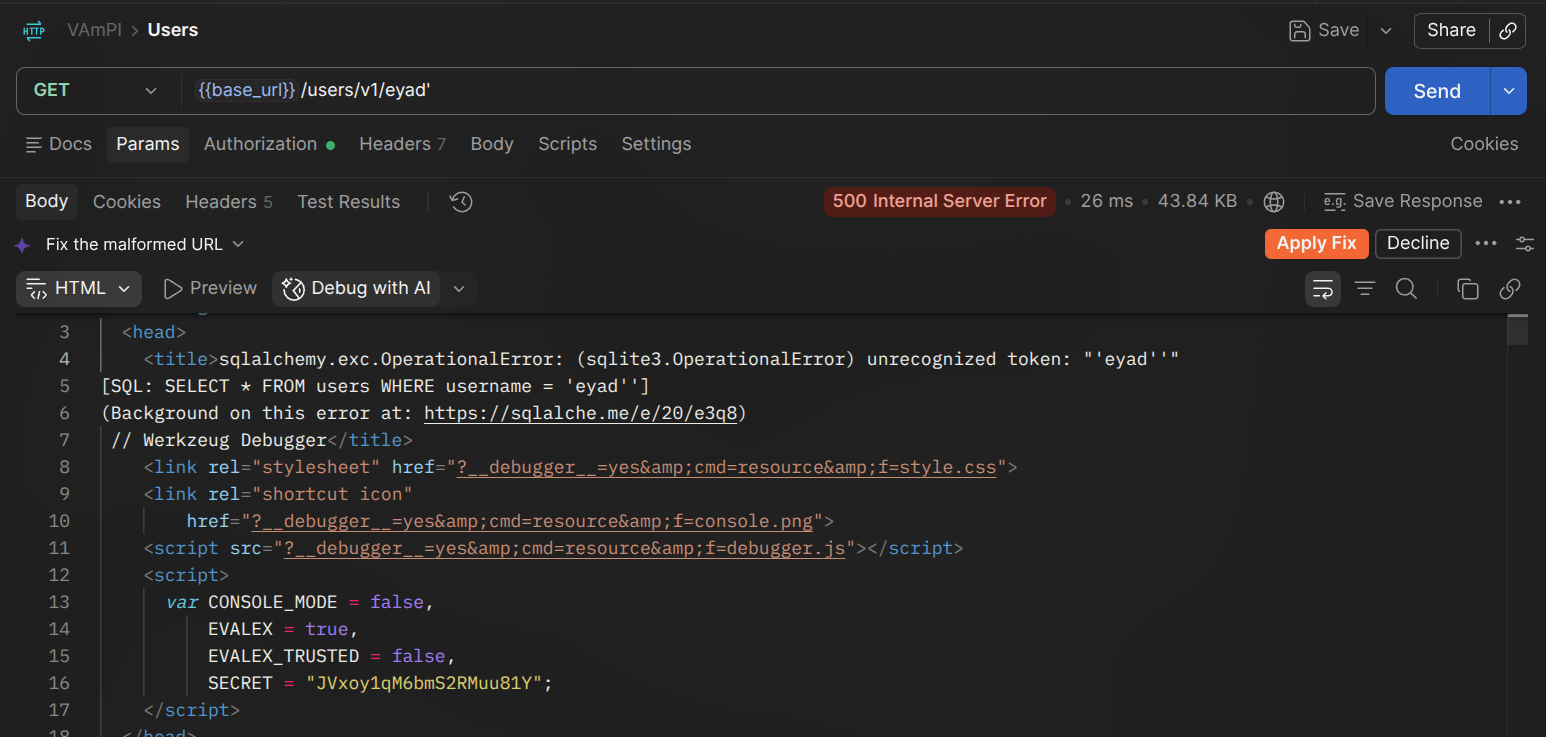
\includegraphics[width=0.92\textwidth]{information disclosure.png}
  \caption{Raw SQL error and Werkzeug debugger secret exposed in the HTTP response body}
\end{figure}

\textbf{Remediation.} Catch all exceptions server-side; return only a generic error message to the client. Disable Werkzeug debug mode (\texttt{DEBUG=False}).

%% ─── Finding 9 ───────────────────────────────────────────────────────────
\subsection{VULN-09 -- User and Credential Enumeration}

\begin{findingbox}{VULN-09: User Enumeration via Public Endpoint}{\medium{MEDIUM}}
\begin{tabular}{ll}
  \textbf{Endpoint}   & \texttt{GET /users/v1} \\
  \textbf{OWASP}      & API9:2023 -- Improper Inventory Management \\
  \textbf{CVSS Score} & 5.3 (AV:N/AC:L/PR:N/UI:N/S:U/C:L/I:N/A:N) \\
\end{tabular}
\end{findingbox}

\textbf{Description.}
The \texttt{/users/v1} endpoint returns a list of all usernames without authentication. Combined with the debug endpoint (VULN-07), complete credential sets are exposed. Even in isolation, the username list fuels targeted brute force (VULN-06).

\textbf{Remediation.}
\begin{itemize}[noitemsep]
  \item Require authentication (at minimum) to list users.
  \item Implement pagination and restrict data returned per role.
\end{itemize}

\newpage
%% ─── Finding 10 ──────────────────────────────────────────────────────────
\subsection{VULN-10 -- Missing Email Format Validation}

\begin{findingbox}{VULN-10: No Email Validation on Registration}{\low{LOW}}
\begin{tabular}{ll}
  \textbf{Endpoint}   & \texttt{POST /users/v1/register} \\
  \textbf{OWASP}      & API3:2023 -- Broken Object Property Level Authorization \\
  \textbf{CVSS Score} & 3.1 (AV:N/AC:H/PR:N/UI:N/S:U/C:N/I:L/A:N) \\
\end{tabular}
\end{findingbox}

\textbf{Description.}
The registration endpoint accepts any string as the email field without format validation or domain verification. Submitting \texttt{"email":"eyad"} returns \texttt{200 OK}.

\begin{figure}[h!]
  \centering
  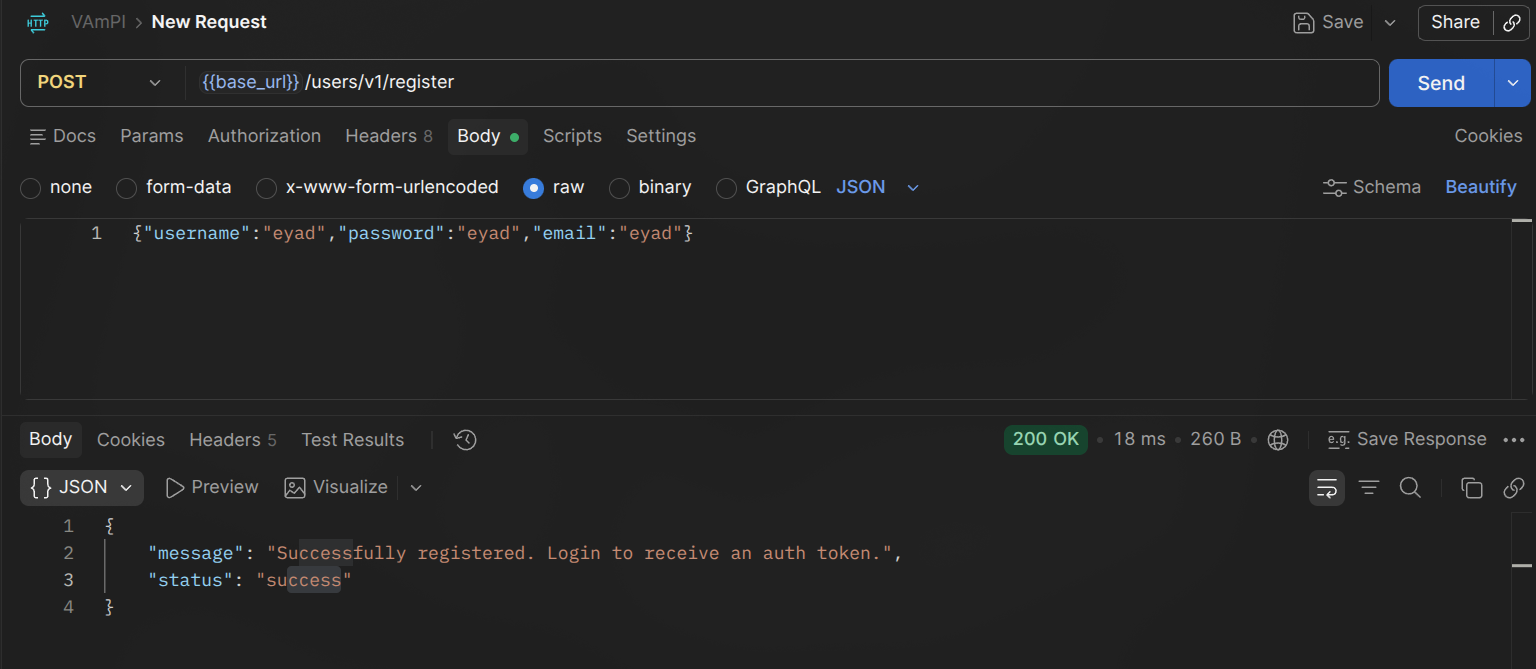
\includegraphics[width=0.88\textwidth]{emailNotVerified.png}
  \caption{Registration succeeds with \texttt{"email":"eyad"} -- no format check performed}
\end{figure}

\textbf{Remediation.}
\begin{itemize}[noitemsep]
  \item Validate email format server-side (regex + DNS MX check).
  \item Implement email ownership verification via confirmation link.
\end{itemize}

%% ─── Finding 11 ──────────────────────────────────────────────────────────
\subsection{VULN-11 -- Weak Password Policy}

\begin{findingbox}{VULN-11: No Minimum Password Strength Enforcement}{\low{LOW}}
\begin{tabular}{ll}
  \textbf{Endpoint}   & \texttt{POST /users/v1/register} \\
  \textbf{OWASP}      & API3:2023 -- Broken Object Property Level Authorization \\
  \textbf{CVSS Score} & 3.7 (AV:N/AC:H/PR:N/UI:N/S:U/C:L/I:N/A:N) \\
\end{tabular}
\end{findingbox}

\textbf{Description.}
Single-character passwords such as \texttt{"password":"a"} are accepted. Pre-existing seeded passwords (\texttt{pass}, \texttt{pass1}, \texttt{pass2}) appear in the first 4,000 entries of \texttt{rockyou.txt}, confirming trivial crackability.

\textbf{Remediation.}
\begin{itemize}[noitemsep]
  \item Enforce minimum length (12+ characters) and complexity or passphrase requirements.
  \item Reject passwords found in known-breached wordlists (HIBP API or local blocklist).
\end{itemize}

\newpage
%% ═══════════════════════════════════════════════════════════════════════════
\section{Risk Matrix}
%% ═══════════════════════════════════════════════════════════════════════════

\begin{center}
\begin{tabular}{lcccc}
  \toprule
  \textbf{Finding} & \textbf{CVSS} & \textbf{Exploitability} & \textbf{Impact} & \textbf{Severity} \\
  \midrule
  VULN-01 SQLi              & 9.8 & Easy   & Full DB dump       & \critical{CRITICAL} \\
  VULN-02 JWT Weak Secret   & 9.1 & Easy   & Auth bypass        & \critical{CRITICAL} \\
  VULN-03 Mass Assignment   & 8.8 & Easy   & Admin escalation   & \high{HIGH} \\
  VULN-04 Unauth Pwd Change & 8.1 & Easy   & Account takeover   & \high{HIGH} \\
  VULN-05 BOLA Books        & 7.5 & Easy   & Data leakage       & \high{HIGH} \\
  VULN-06 Brute Force       & 7.5 & Easy   & Credential theft   & \high{HIGH} \\
  VULN-07 Debug Endpoint    & 6.5 & Easy   & Full cred dump     & \medium{MEDIUM} \\
  VULN-08 Info Disclosure   & 5.3 & Easy   & Recon aid          & \medium{MEDIUM} \\
  VULN-09 User Enumeration  & 5.3 & Easy   & Username harvest   & \medium{MEDIUM} \\
  VULN-10 No Email Verify   & 3.1 & Medium & Spam / fake accts  & \low{LOW} \\
  VULN-11 Weak Password     & 3.7 & Medium & Brute force risk   & \low{LOW} \\
  \bottomrule
\end{tabular}
\end{center}

%% ═══════════════════════════════════════════════════════════════════════════
\section{Remediation Roadmap}
%% ═══════════════════════════════════════════════════════════════════════════

\begin{center}
\begin{tabularx}{\textwidth}{clXl}
  \toprule
  \textbf{Priority} & \textbf{Finding} & \textbf{Remediation} & \textbf{Effort} \\
  \midrule
  1 & VULN-01 & Parameterised queries; disable debug mode       & Low \\
  2 & VULN-02 & Regenerate JWT secret with CSPRNG (256-bit)     & Low \\
  3 & VULN-03 & Input allowlist on registration model           & Low \\
  4 & VULN-04 & Object-level authorisation check on PUT handler & Low \\
  5 & VULN-05 & Owner check before returning book secret        & Low \\
  6 & VULN-06 & Rate limiting + account lockout on login        & Medium \\
  7 & VULN-07 & Remove debug endpoint from production           & Low \\
  8 & VULN-08 & Generic error handler; \texttt{DEBUG=False}     & Low \\
  9 & VULN-09 & Require auth for user listing                   & Low \\
  10 & VULN-10 & Server-side email format validation            & Low \\
  11 & VULN-11 & Minimum password policy + blocklist            & Low \\
  \bottomrule
\end{tabularx}
\end{center}

%% ═══════════════════════════════════════════════════════════════════════════
\section{Conclusion}
%% ═══════════════════════════════════════════════════════════════════════════

VAmPI exhibits a severe and comprehensive set of API security weaknesses. Two \textbf{Critical} vulnerabilities -- SQL Injection and weak JWT secret -- independently allow full system compromise with minimal effort. All 11 findings have straightforward remediations that require no architectural changes, primarily input validation, authorisation checks, and secure configuration.

\vspace{1em}
\begin{tcolorbox}[colback=critred!10,colframe=critred,title=\textbf{Immediate Action Required}]
Findings VULN-01 through VULN-04 must be remediated before any production deployment. VULN-07 (debug endpoint) should be removed immediately as it provides instant full credential disclosure without authentication.
\end{tcolorbox}



\end{document}
